\documentclass{training}
\schoollogo{../../resources/intros/UI-00-colors-and-moodboard.jpg}
\setlang{french}
\newcommand{\uxfond}{../../resources/fond/UI-00-colors-and-moodboard.png}
% Filigrane PAR MODULE : \uxfond (PNG A4 dilue 30 %). Cadre noir vectoriel commun.
% Proportions original 744 px : marge 20/744, trait 1/744. Exterieur BLANC.
% Cadre via eso-pic +\put (coordonnees absolues) — pas de remember picture (decalage).
\usepackage{eso-pic}

\providecommand{\uxfond}{../../resources/fond/norme_fond_paliers_30.png}

\newlength{\uxmargin}
\newlength{\uxthick}
\newlength{\uxinnerw}
\newlength{\uxinnerh}
\setlength{\uxmargin}{0.02688\paperwidth}% 20/744
\setlength{\uxthick}{0.001344\paperwidth}% 1/744
\setlength{\uxinnerw}{\dimexpr\paperwidth-2\uxmargin-2\uxthick\relax}
\setlength{\uxinnerh}{\dimexpr\paperheight-2\uxmargin-2\uxthick\relax}

% Contenu strictement a l'interieur du trait (+ jour confortable).
\geometry{%
  includeheadfoot,
  left=22mm,
  right=22mm,
  top=20mm,
  bottom=18mm,
  headheight=30pt,
  headsep=5mm,
  footskip=12mm%
}

\AddToShipoutPictureBG{%
  \AtPageLowerLeft{%
    % Fond blanc page entiere
    \put(0,0){\color{white}\rule{\paperwidth}{\paperheight}}%
    % Filigrane module a l'interieur du cadre
    \put(\LenToUnit{\dimexpr\uxmargin+\uxthick\relax},\LenToUnit{\dimexpr\uxmargin+\uxthick\relax}){%
      \includegraphics[width=\uxinnerw,height=\uxinnerh]{\uxfond}}%
    % Cadre noir : bas, haut, gauche, droite
    \put(\LenToUnit{\uxmargin},\LenToUnit{\uxmargin}){%
      \color{black}\rule{\dimexpr\paperwidth-2\uxmargin\relax}{\uxthick}}%
    \put(\LenToUnit{\uxmargin},\LenToUnit{\dimexpr\paperheight-\uxmargin-\uxthick\relax}){%
      \color{black}\rule{\dimexpr\paperwidth-2\uxmargin\relax}{\uxthick}}%
    \put(\LenToUnit{\uxmargin},\LenToUnit{\uxmargin}){%
      \color{black}\rule{\uxthick}{\dimexpr\paperheight-2\uxmargin\relax}}%
    \put(\LenToUnit{\dimexpr\paperwidth-\uxmargin-\uxthick\relax},\LenToUnit{\uxmargin}){%
      \color{black}\rule{\uxthick}{\dimexpr\paperheight-2\uxmargin\relax}}%
  }%
}

\makeatletter
\fancyhf{}
\fancyheadoffset{0pt}
\renewcommand{\headrulewidth}{0pt}
\lhead{\parbox[t]{0.56\textwidth}{\RaggedRight\footnotesize\sloppy\@title}}
\rhead{\parbox[t]{0.36\textwidth}{\RaggedLeft\footnotesize\sloppy\@subtitle}}
\cfoot{\thepage}
% Coupures : underscore et slash dans les noms de fichiers / consignes
\DeclareRobustCommand{\_}{\textunderscore\allowbreak}
\makeatother

% Evite les depassements de longues lignes (Github, Name_FirstName_...)
\sloppy
\emergencystretch=3em
\hbadness=10000

% Sommaire type 42 : chapitres seulement
\setcounter{tocdepth}{0}
\renewcommand{\cftchappresnum}{}
\renewcommand{\cftchapaftersnum}{}
\setlength{\cftchapnumwidth}{2.0em}
\setlength{\cftbeforechapskip}{0.35em}
\cftsetindents{chapter}{0em}{2.0em}


\begin{document}

\title{Couleurs et planche d'ambiance}
\subtitle{Piscine UX/UI --- UI}
\member{Piscine UX/UI}{https://github.com/01-edu/UX-UI}
\summary{Couleur, caractère, une planche, et cinq défis d'interface.}
\version{1.0}
\prerequisite{Le module précédent de cette piscine, ou aucun si c'est le premier.}
\maketitle

\newpage
\tableofcontents
\newpage


\chapter{Instructions}

L'avant-propos n'est pas un exercice. Il ne sera pas noté. Les exercices commencent au chapitre suivant, du contrat le plus simple au plus dur. Un exercice plus tardif n'est pas pris en compte si un plus tôt ne tient pas.

On ne regarde que ce qui est dans le répertoire de rendu de l'exercice. N'ajoutez pas un fichier que l'exercice ne nomme pas. Le nom d'un livrable suit le motif imprimé dans l'exercice : \texttt{Name\_FirstName\_DeliverableName\_Date\_VersionNumber}.

Le geste ne vous est pas donné. Les exemples d'un exercice portent parfois une contrainte que la phrase ne répète pas. Lisez-les. Vos autres références sont le manuel de l'outil choisi, la personne assise à côté, et les liens imprimés dans l'exercice.

L'ordre est celui de la quête. Sauter une étape parce qu'un écran plus tard semble plus intéressant produit un écran que personne ne sait expliquer.

\subsection*{Des images}

La marque en couverture est l'image de ce module. Les paliers pâles derrière le texte sont le fond de page. Ni l'un ni l'autre n'est un indice.

\subsection*{Des machines qui écrivent}

Vous pouvez vous servir d'un outil pour vérifier un mot, comme d'un dictionnaire. Vous ne pouvez pas remplacer un entretien, un test ou un fichier par un texte généré et le signer. Si vous ne pouvez pas montrer la personne, l'écran ou la ligne que vous avancez, l'exercice n'est pas fait.


\chapter{Avant-propos}

Josef Albers a passé un livre à montrer qu'une couleur n'est pas une pastille, c'est ce que le voisin lui fait (\emph{Interaction of Color}, Yale University Press, 1963). Johannes Itten l'avait déjà montré avec du papier au Bauhaus. Les défis qui suivent sont des dessins chronométrés. Albers ne les peint pas à votre place.

\begin{center}
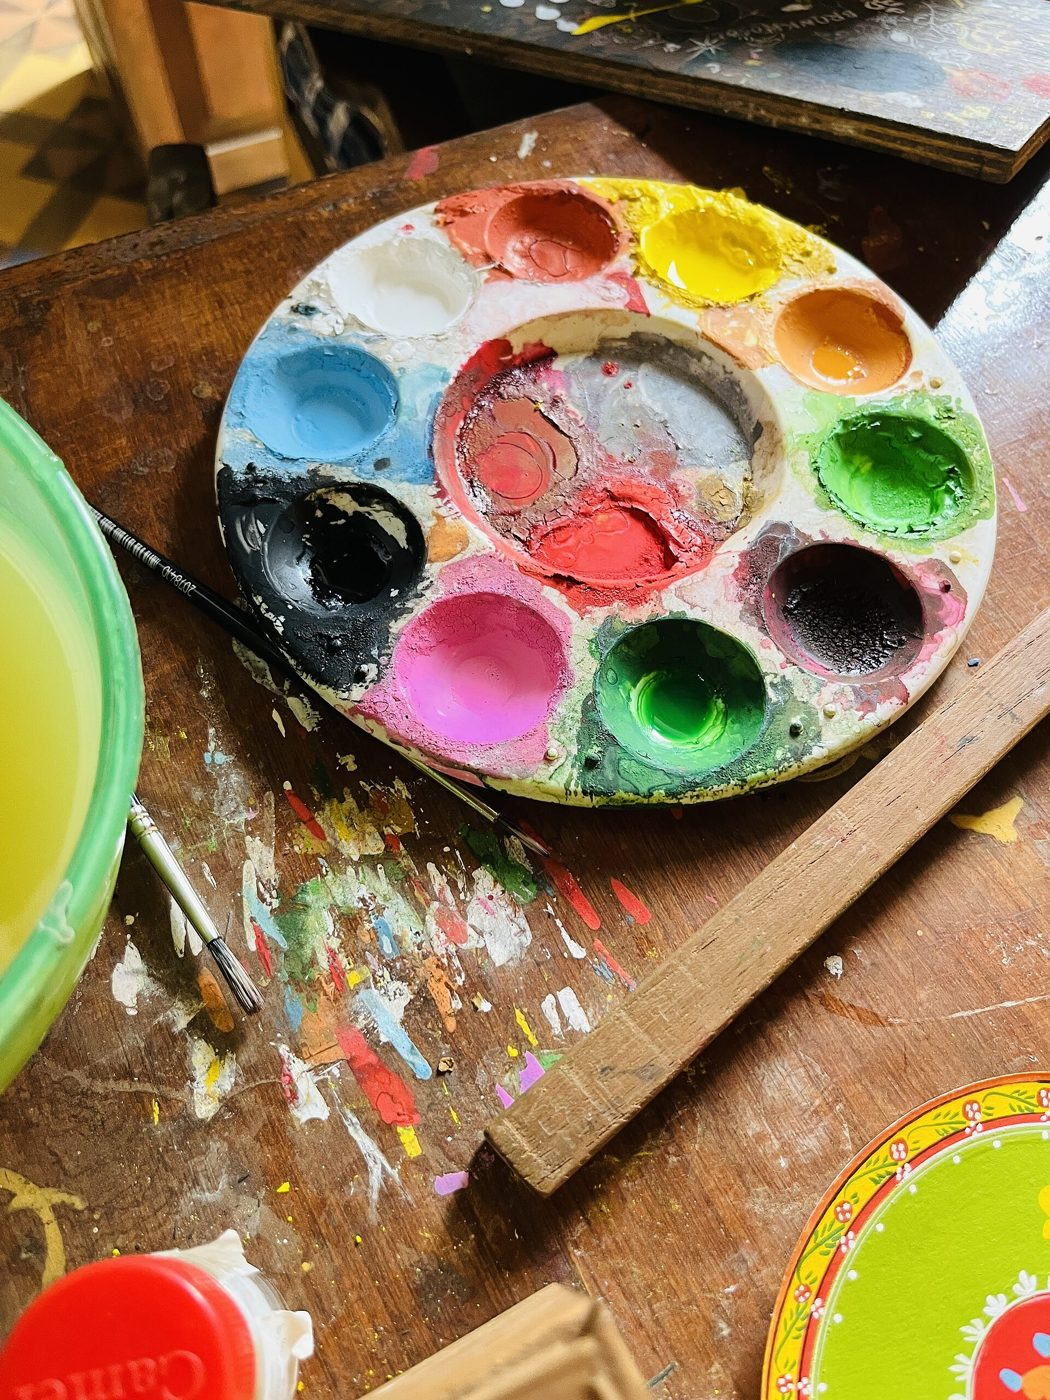
\includegraphics[width=0.78\textwidth,height=0.32\textheight,keepaspectratio]{../../resources/intros/UI-00-colors-and-moodboard.jpg}\\[0.4em]
{\footnotesize Image : Art Projects MKCL KF, CC BY-SA 4.0}
\end{center}

À regarder. Les vidéos sont un contexte. Elles ne sont pas le livrable.
\begin{itemize}
\item UI - Introduction \& Quest n°1, 01Edu \url{https://www.youtube.com/watch?v=UbE6WMeuvQg&list=PLHyAJ_GrRtf-_aBft2jQL4-QAunn2bLvu}
\end{itemize}

\chapter{Exercice 00 : UI I - Ex 1 - Trouver les couleurs}
\exnumber{00}
\extitle{UI I - Ex 1 - Trouver les couleurs}
\exfiles{ex00/fichier Figma et PDF, nomme Name\_FirstName\_DeliverableName\_Date\_VersionNumber}
\exauthorize{Ceux nommés dans l'exercice}
\makeheaderfiles

\textbf{Contexte :}

Cette première quête UI est une série d'exercices pour pratiquer les couleurs, les moodboards, la typographie et reproduire des écrans sur Figma !

\textbf{Instructions :}

Allez sur ces 7 sites web et créez les palettes de couleurs à partir d'eux (3 à 4 couleurs principales).

\textbf{Livrable :}

\begin{itemize}
\item Un fichier Figma comprenant des captures de la page principale, l'URL et les couleurs extraites à côté des captures.
\item Déposez le fichier Figma sur Github, nommé ainsi : « Name\_FirstName\_DeliverableName\_Date\_VersionNumber ». Exemple : « Doe\_John\_MidFiPrototype\_05242024\_V1 ».
\item Ajoutez un titre dans le fichier.
\item Soignez l'aspect global du fichier. Il doit être clair, simple et lisible. Vous pouvez regarder canva.com, sans surcharger le dessin de détails.
\end{itemize}

\textbf{Pistes :}

\begin{itemize}
\item Vous pouvez utiliser Figma pour extraire les couleurs dont vous avez besoin et exporter votre fichier en PDF.
\item Utilisez la pipette de couleur pour extraire les couleurs !
\item Vous pouvez montrer les couleurs principales avec des carrés ou des cercles remplis à côté des captures d'écran.
\item Soignez l'esthétique de votre livrable ! 1 page par site devrait convenir.
\end{itemize}

\begin{itemize}
\item https://www.komoot.com/ \url{https://www.komoot.com/} (App)
\item https://www.airtable.com/ \url{https://www.airtable.com/}
\item https://www.decathlon.com/collections/kids-gift-ideas \url{https://www.decathlon.com/collections/kids-gift-ideas}
\item https://www.jrpass.com/ \url{https://www.jrpass.com/}
\item https://www.thesiff.com/ \url{https://www.thesiff.com/}
\item https://brave.com/es/ \url{https://brave.com/es/}
\item https://www.nhp.gov.in/ \url{https://www.nhp.gov.in/}
\end{itemize}

\textbf{Ressources :}

\begin{itemize}
\item Tutoriel vidéo sur Figma \url{https://www.youtube.com/watch?v=FTFaQWZBqQ8}
\item Débuter en design graphique \url{https://edu.gcfglobal.org/en/beginning-graphic-design/}
\item Gareth graphic studio \url{https://www.youtube.com/c/GarethDavidStudio}
\end{itemize}


\chapter{Exercice 01 : UI I - Ex 2 - Codes couleur}
\exnumber{01}
\extitle{UI I - Ex 2 - Codes couleur}
\exfiles{ex01/fichier Figma, nomme Name\_FirstName\_DeliverableName\_Date\_VersionNumber}
\exauthorize{Ceux nommés dans l'exercice}
\makeheaderfiles

\textbf{Instructions :}

Allez sur ces 7 sites web et créez les palettes de couleurs à partir d'eux (3 à 4 couleurs principales).

\textbf{Livrable :}

\begin{itemize}
\item Un fichier Figma comprenant des captures de la page principale, l'URL, les couleurs extraites et les codes couleur correspondants.
\item Déposez le fichier Figma sur Github, nommé ainsi : « Name\_FirstName\_DeliverableName\_Date\_VersionNumber ». Exemple : « Doe\_John\_MidFiPrototype\_05242024\_V1 ».
\item Ajoutez un titre dans le fichier.
\item Soignez l'aspect global du fichier. Il doit être clair, simple et lisible. Vous pouvez regarder canva.com, sans surcharger le dessin de détails.
\end{itemize}

\textbf{Pistes :}

\begin{itemize}
\item Vous pouvez utiliser le document de l'exercice précédent pour ajouter les codes couleur sur Figma.
\item Utilisez la pipette de couleur pour détecter les codes couleur !
\end{itemize}

\textbf{Ressources :}

\begin{itemize}
\item Débuter en design graphique \url{https://edu.gcfglobal.org/en/beginning-graphic-design/}
\item Gareth graphic studio \url{https://www.youtube.com/c/GarethDavidStudio}
\end{itemize}

\begin{itemize}
\item https://www.komoot.com/ \url{https://www.komoot.com/} (App)
\item https://www.airtable.com/ \url{https://www.airtable.com/}
\item https://www.decathlon.com/collections/kids-gift-ideas \url{https://www.decathlon.com/collections/kids-gift-ideas}
\item https://www.jrpass.com/ \url{https://www.jrpass.com/}
\item https://www.thesiff.com/ \url{https://www.thesiff.com/}
\item https://brave.com/es/ \url{https://brave.com/es/}
\item https://www.nhp.gov.in/ \url{https://www.nhp.gov.in/}
\end{itemize}


\chapter{Exercice 02 : UI I - Ex 3 - Combinaisons de couleurs}
\exnumber{02}
\extitle{UI I - Ex 3 - Combinaisons de couleurs}
\exfiles{ex02/fichier Figma, nomme Name\_FirstName\_DeliverableName\_Date\_VersionNumber}
\exauthorize{Those named in the exercise}
\makeheaderfiles

\textbf{Instructions :}

Let's browse!

Find 3 digital products (websites or apps) that use each kind of color palette combination:

\begin{itemize}
\item Monochromatic
\item Analogous
\item Complementary
\item Split complementary
\item Triadic
\item Double complementary
\end{itemize}

\textbf{Livrable :}

\begin{itemize}
\item A Figma file including for each digital product (websites or apps)
\begin{itemize}
\item screenshots of the main page
\item the matching URL
\item the main colors and
\item the kind of color combination.
\end{itemize}
\item Déposez le fichier Figma sur Github, nommé ainsi : « Name\_FirstName\_DeliverableName\_Date\_VersionNumber ». Exemple : « Doe\_John\_MidFiPrototype\_05242024\_V1 ».
\item Ajoutez un titre dans le fichier.
\item Soignez l'aspect global du fichier. Il doit être clair, simple et lisible. Vous pouvez regarder canva.com, sans surcharger le dessin de détails.
\end{itemize}

\textbf{Pistes :}

\begin{itemize}
\item You can find HSB (Hue, Saturation, Brightness) as well as HSV (Hue, Saturation, Value) depending of the source.
\end{itemize}

\textbf{Ressources :}

\begin{itemize}
\item https://coloursandmaterials.wordpress.com/2014/09/16/colour-system/ \url{https://coloursandmaterials.wordpress.com/2014/09/16/colour-system/}
\item Color wheel combinations
\end{itemize}

\textbf{Monochromatic examples:}

\begin{itemize}
\item https://www.benefitcosmetics.com/ \url{https://www.benefitcosmetics.com/} 
\item http://www.jwilouvres.com.au/ \url{http://www.jwilouvres.com.au/} 
\item http://blank.com.pt/ \url{http://blank.com.pt/}
\end{itemize}

\textbf{Analogous examples:}

\begin{itemize}
\item https://www.natuurenmilieu.nl/ \url{https://www.natuurenmilieu.nl/} 
\item https://campesinorum.com/ \url{https://campesinorum.com/} 
\item https://www.lobster.es/ \url{https://www.lobster.es/}
\end{itemize}

\textbf{Complementary examples:}

\begin{itemize}
\item https://www.rolandgarros.com/ \url{https://www.rolandgarros.com/fr-fr} 
\item https://squilla.io/ \url{https://squilla.io/} 
\item https://gomim.com/en/ \url{https://gomim.com/en/}
\end{itemize}

\textbf{Split complementary examples:}

\begin{itemize}
\item https://flythenest.io/en/ \url{https://flythenest.io/en/} 
\item https://www.kineuphorics.com/ \url{https://www.kineuphorics.com/} 
\item https://www.ma-tea.de/ \url{https://www.ma-tea.de/}
\end{itemize}

\textbf{Triadic examples}

\begin{itemize}
\item https://normalnow.com/ \url{https://normalnow.com/} 
\item https://brainbakery.com/en/ \url{https://brainbakery.com/en/} 
\item https://www.barkbox.com/ \url{https://www.barkbox.com/}
\end{itemize}

\textbf{Dual complementary or Tetradic examples}

\begin{itemize}
\item https://www.airtable.com/ \url{https://www.airtable.com/} 
\item https://calendar.google.com/ \url{https://calendar.google.com/} 
\item https://www.ebay.com/ \url{https://www.ebay.com/}
\end{itemize}


\chapter{Exercice 03 : UI I - Ex 4 - Planche d'ambiance}
\exnumber{03}
\extitle{UI I - Ex 4 - Planche d'ambiance}
\exfiles{ex03/fichier Figma, nomme Name\_FirstName\_DeliverableName\_Date\_VersionNumber}
\exauthorize{Ceux nommés dans l'exercice}
\makeheaderfiles

\textbf{Instructions :}

Créez 4 moodboards différents à partir de ces 4 briefs et extrayez une palette de couleurs.

\textbf{Briefs :}

\begin{itemize}
\item 1 : Un professeur de physique qui veut rendre son site accrocheur pour des enfants de 12 ans.
\item 2 : Un site de wedding planner sri-lankais qui veut respirer sobriété et modernité.
\item 3 : Une plateforme e-commerce qui vend du wax ouest-africain et veut paraître plus luxueuse dans son esprit pour se démarquer.
\item 4 : Une ONG qui aide les parents d'enfants autistes, veut diffuser joie et espoir pour une collecte de fonds.
\end{itemize}

\textbf{Livrables :}

\begin{itemize}
\item Un fichier Figma par planche d'ambiance
\item Sur chaque moodboard, plusieurs images (5 à 12) graphiquement cohérentes en termes de couleurs
\item Les couleurs principales extraites et affichées sur le côté
\item Un code couleur par couleur (RVB, Hex ou HSB)
\item Déposez les documents sur Github, dans un zip nommé « ProjectTitle\_Name\_FirstName », et chaque livrable ainsi : « Name\_FirstName\_DeliverableName\_Date\_VersionNumber ». Exemple : « Doe\_John\_MidFiPrototype\_05242024\_V1 ».
\item Ajoutez un titre dans tous les documents écrits.
\item Soignez l'aspect global des livrables. Ils doivent être clairs, simples et lisibles. Vous pouvez regarder canva.com, sans surcharger le dessin de détails.
\end{itemize}

\textbf{Pistes :}

\begin{itemize}
\item Utilisez des images librement utilisables ! \url{https://buffer.com/library/free-images/}
\item Exemples de moodboards (en plus, le moodboard doit inclure les codes couleur) :
\item https://lovestylecomunicacion.com/wp-content/uploads/2017/09/A.png \url{https://lovestylecomunicacion.com/wp-content/uploads/2017/09/A.png}
\item https://caseperlatesta.com/wp-content/uploads/2015/09/Moodboard23\_grey\_peach-1024x1024.jpg \url{https://caseperlatesta.com/wp-content/uploads/2015/09/Moodboard23_grey_peach-1024x1024.jpg}
\item https://i.pinimg.com/564x/ee/9d/d6/ee9dd6fbb82b0e5b4dd2924580b765dd.jpg \url{https://i.pinimg.com/564x/ee/9d/d6/ee9dd6fbb82b0e5b4dd2924580b765dd.jpg}
\end{itemize}


\chapter{Exercice 04 : UI I - Ex 5 - Typographie}
\exnumber{04}
\extitle{UI I - Ex 5 - Typographie}
\exfiles{ex04/fichier Figma, nomme Name\_FirstName\_DeliverableName\_Date\_VersionNumber}
\exauthorize{Ceux nommés dans l'exercice}
\makeheaderfiles

\textbf{Instructions :}

Allez sur ces sites web et détectez les typographies utilisées.

\begin{itemize}
\item https://unric.org/no \url{https://unric.org/no}
\item https://www.strongbowcider.com/bug-exterminator-brisbane \url{https://www.strongbowcider.com/bug-exterminator-brisbane}
\item http://www.bbqgrillsandfire.com/ \url{http://www.bbqgrillsandfire.com/}
\item https://pt.wikipedia.org/wiki/Mario\_Botta \url{https://pt.wikipedia.org/wiki/Mario_Botta}
\item https://texas-private-investigator.com/ \url{https://texas-private-investigator.com/}
\item https://bumble.com/ \url{https://bumble.com/}
\item https://adopte1poule.fr/ \url{https://adopte1poule.fr/}
\item http://slaveryfootprint.org/ \url{http://slaveryfootprint.org/}
\item https://www.tomorrowland.com/fr/festival/bienvenue \url{https://www.tomorrowland.com/fr/festival/bienvenue}
\item https://artisanscanada.com/ \url{https://artisanscanada.com/}
\end{itemize}

\textbf{Livrables :}

\begin{itemize}
\item Un fichier Figma montrant toutes les typographies utilisées dans chaque site ou application.
\item Déposez le fichier Figma sur Github, nommé ainsi : « Name\_FirstName\_DeliverableName\_Date\_VersionNumber ». Exemple : « Doe\_John\_MidFiPrototype\_05242024\_V1 ».
\item Ajoutez un titre dans le fichier.
\item Soignez l'aspect global du fichier. Il doit être clair, simple et lisible. Vous pouvez regarder canva.com, sans surcharger le dessin de détails.
\end{itemize}

\textbf{Pistes :}

\begin{itemize}
\item Soignez la présentation !
\item N'hésitez pas à parcourir les options de Google Chrome pour détecter la typographie ;-)
\item Google Fonts \url{https://fonts.google.com/} est un autre excellent allié à avoir à vos côtés
\end{itemize}

\textbf{Ressources :}

\begin{itemize}
\item Qu'est-ce que la typographie \url{https://www.renderforest.com/blog/what-is-typography}
\item Pourquoi la typographie est-elle importante ? \url{https://careerfoundry.com/en/blog/ui-design/beginners-guide-to-typography/}
\item Débuter en design graphique : Typographie \url{https://edu.gcfglobal.org/en/beginning-graphic-design/typography/1/}
\item Débuter en design graphique \url{https://edu.gcfglobal.org/en/beginning-graphic-design/}
\item Gareth graphic studio \url{https://www.youtube.com/c/GarethDavidStudio}
\end{itemize}


\chapter{Exercice 05 : UI I - Ex 6 - Planche typographique}
\exnumber{05}
\extitle{UI I - Ex 6 - Planche typographique}
\exfiles{ex05/fichier Figma, nomme Name\_FirstName\_DeliverableName\_Date\_VersionNumber}
\exauthorize{Those named in the exercise}
\makeheaderfiles

\textbf{Instructions :}

Find consistent typography for your moodboards from Ex. 4.

\textbf{Livrables :}

\begin{itemize}
\item A Figma file with 4 moodboards from Ex. 4 and typography:
\begin{itemize}
\item 1 for a title
\item 1 for a button
\item 1 for a description
\item 1 for the text
\end{itemize}
\item Déposez le fichier Figma sur Github, nommé ainsi : « Name\_FirstName\_DeliverableName\_Date\_VersionNumber ». Exemple : « Doe\_John\_MidFiPrototype\_05242024\_V1 ».
\item Ajoutez un titre dans le fichier.
\item Soignez l'aspect global du fichier. Il doit être clair, simple et lisible. Vous pouvez regarder canva.com, sans surcharger le dessin de détails.
\end{itemize}

\textbf{Ressources :}

\begin{itemize}
\item Font \url{https://en.wikipedia.org/wiki/Font}
\item Glyph \url{https://en.wikipedia.org/wiki/Glyph}
\item Instagram account: You are typography \url{https://www.instagram.com/youaretypography/}
\item Instagram account: Typespire \url{https://www.instagram.com/typespire/}
\item Instagram account: ux\_ui.world \url{https://www.instagram.com/ui_ux.world/}
\item Instagram account: ui.netwrk \url{https://www.instagram.com/ui.netwrk/}
\item Instagram account: uxuidailytips \url{https://www.instagram.com/uiuxdailytips/}
\end{itemize}

\textbf{Pistes :}

\begin{itemize}
\item Bold, italic, normal, light, etc. are fonts, not typography.
\item Google Fonts \url{https://fonts.google.com/} is another great friend to have by your side
\item Example of a caption here \url{https://www.figma.com/file/SbQMPjfLOzg92g8YZFlrRh/UI-I---Ex-5}
\end{itemize}

\textbf{Ressources :}

\begin{itemize}
\item What is Typography \url{https://www.renderforest.com/blog/what-is-typography}
\item Why is Typography important? \url{https://careerfoundry.com/en/blog/ui-design/beginners-guide-to-typography/}
\item Beginning graphic design: Typography \url{https://edu.gcfglobal.org/en/beginning-graphic-design/typography/1/}
\item Beginning graphic design \url{https://edu.gcfglobal.org/en/beginning-graphic-design/}
\item Gareth graphic studio \url{https://www.youtube.com/c/GarethDavidStudio}
\end{itemize}


\chapter{Exercice 06 : UI I - Ex 7 - Défi UI - Minuteur}
\exnumber{06}
\extitle{UI I - Ex 7 - Défi UI - Minuteur}
\exfiles{ex06/fichier Figma, nomme Name\_FirstName\_DeliverableName\_Date\_VersionNumber}
\exauthorize{Those named in the exercise}
\makeheaderfiles

\textbf{Instructions :}

Copy this image on Figma.
Timer

\textbf{Livrable :}

\begin{itemize}
\item A Figma file
\item Please make sure you use:
\begin{itemize}
\item 2 half circles to draw the circle around the timer
\item Gradient to fill the main circle
\item Groups
\item Named layers
\end{itemize}
\item Déposez le fichier Figma sur Github, nommé ainsi : « Name\_FirstName\_DeliverableName\_Date\_VersionNumber ». Exemple : « Doe\_John\_MidFiPrototype\_05242024\_V1 ».
\item Ajoutez un titre dans le fichier.
\item Soignez l'aspect global du fichier. Il doit être clair, simple et lisible. Vous pouvez regarder canva.com, sans surcharger le dessin de détails.
\end{itemize}

\textbf{Pistes :}

\begin{itemize}
\item The font is RAJDANHI
\item The frame is Android 360 x 640px
\end{itemize}


\chapter{Exercice 07 : UI I - Ex 8 - Défi UI - Montres}
\exnumber{07}
\extitle{UI I - Ex 8 - Défi UI - Montres}
\exfiles{ex07/fichier Figma, nomme Name\_FirstName\_DeliverableName\_Date\_VersionNumber}
\exauthorize{Ceux nommés dans l'exercice}
\makeheaderfiles

\textbf{Instructions :}

Copiez ces images sur Figma

Screen1
Screen2
Screen3
Screen4

\textbf{Livrable :}

\begin{itemize}
\item Un fichier Figma avec une copie de l'image et des éléments Figma
\item Vérifiez :
\begin{itemize}
\item Vous utilisez des symboles et des variants
\item Tous vos calques sont nommés et organisés
\item Vous utilisez des overlays
\item Vous utilisez des masques pour changer la forme de l'image importée
\end{itemize}
\item Déposez le fichier Figma sur Github, nommé ainsi : « Name\_FirstName\_DeliverableName\_Date\_VersionNumber ». Exemple : « Doe\_John\_MidFiPrototype\_05242024\_V1 ».
\item Ajoutez un titre dans le fichier.
\item Soignez l'aspect global du fichier. Il doit être clair, simple et lisible. Vous pouvez regarder canva.com, sans surcharger le dessin de détails.
\end{itemize}

\textbf{Pistes :}

\begin{itemize}
\item Polices : SF Compact pour les éléments iOS, Futura STD Condensed pour les signes Nike
\item Le frame pour chaque écran iWatch est watch 44 mm 184 x 224
\item Article Figma sur les Symbols et Variants \url{https://help.figma.com/hc/en-us/articles/360056440594-Create-and-use-variants}
\item Vous pouvez utiliser des Libraries existantes en parcourant les ressources de la communauté Figma
\end{itemize}


\chapter{Exercice 08 : UI I - Ex 9 - Défi UI - Vol}
\exnumber{08}
\extitle{UI I - Ex 9 - Défi UI - Vol}
\exfiles{ex08/fichier Figma, nomme Name\_FirstName\_DeliverableName\_Date\_VersionNumber}
\exauthorize{Those named in the exercise}
\makeheaderfiles

\textbf{Instructions}:

Copiez cette image dans Figma

Flight

\textbf{Livrable :}

\begin{itemize}
\item Un fichier Figma avec une copie de l'image et des éléments Figma
\item Vérifiez :
\begin{itemize}
\item Vous utilisez des symboles et des variants
\item All you layers are names and organized
\item Vous utilisez des overlays
\item You use masks to change the shape of an imported image (Amsterdam, Maldives, New Delhi, Sydney icons)
\end{itemize}
\item Déposez le fichier Figma sur Github, nommé ainsi : « Name\_FirstName\_DeliverableName\_Date\_VersionNumber ». Exemple : « Doe\_John\_MidFiPrototype\_05242024\_V1 ».
\item Ajoutez un titre dans le fichier.
\item Soignez l'aspect global du fichier. Il doit être clair, simple et lisible. Vous pouvez regarder canva.com, sans surcharger le dessin de détails.
\end{itemize}

\textbf{Pistes :}

\begin{itemize}
\item Font: Roboto Bold, Normal, Black with 0 to 7\% space between letters
\item The frame is desktop 1440 x 1048 px
\item Figma article about Symbols and Variants \url{https://help.figma.com/hc/en-us/articles/360056440594-Create-and-use-variants}
\end{itemize}


\chapter{Exercice 09 : UI I - Ex 10 - Défi UI - Spotify}
\exnumber{09}
\extitle{UI I - Ex 10 - Défi UI - Spotify}
\exfiles{ex09/fichier Figma, nomme Name\_FirstName\_DeliverableName\_Date\_VersionNumber}
\exauthorize{Those named in the exercise}
\makeheaderfiles

\textbf{Instructions :}

Copiez cette image dans Figma
Spotify

\textbf{Livrable :}

\begin{itemize}
\item Un fichier Figma avec une copie de l'image et des éléments Figma
\item Please make sure you use:
\begin{itemize}
\item Linear color background
\item Groups
\item Named and organized layers
\item Apple design system (head bar)
\item Symbols and variants for the songs (1 page for the Symbols)
\end{itemize}
\item Déposez le fichier Figma sur Github, nommé ainsi : « Name\_FirstName\_DeliverableName\_Date\_VersionNumber ». Exemple : « Doe\_John\_MidFiPrototype\_05242024\_V1 ».
\item Ajoutez un titre dans le fichier.
\item Soignez l'aspect global du fichier. Il doit être clair, simple et lisible. Vous pouvez regarder canva.com, sans surcharger le dessin de détails.
\end{itemize}

\textbf{Pistes :}

\begin{itemize}
\item The font is GOTHAM
\item The frame is iPhone 13 Pro Max 428 x 926 px
\item Figma article about Symbols and Variants \url{https://help.figma.com/hc/en-us/articles/360056440594-Create-and-use-variants}
\end{itemize}


\chapter{Exercice 10 : UI I - Ex 11 - Défi UI - Tableau de bord Bitcoin}
\exnumber{10}
\extitle{UI I - Ex 11 - Défi UI - Tableau de bord Bitcoin}
\exfiles{ex10/fichier Figma, nomme Name\_FirstName\_DeliverableName\_Date\_VersionNumber}
\exauthorize{Those named in the exercise}
\makeheaderfiles

\textbf{Instructions :}

Copiez cette image dans Figma
Dashboard

\textbf{Livrable :}

\begin{itemize}
\item Un fichier Figma avec une copie de l'image et des éléments Figma
\item Vérifiez :
\begin{itemize}
\item Vous utilisez des symboles et des variants
\item All your layers are named and organized
\item Vous utilisez des overlays
\item You use masks to change the shape of an imported image
\item You use linear color function
\end{itemize}
\item Déposez le fichier Figma sur Github, nommé ainsi : « Name\_FirstName\_DeliverableName\_Date\_VersionNumber ». Exemple : « Doe\_John\_MidFiPrototype\_05242024\_V1 ».
\item Ajoutez un titre dans le fichier.
\item Soignez l'aspect global du fichier. Il doit être clair, simple et lisible. Vous pouvez regarder canva.com, sans surcharger le dessin de détails.
\end{itemize}

\textbf{Pistes :}

\begin{itemize}
\item Fonts: Avenir
\item The frame is a desktop 1440 x 1024
\item Figma article about Symbols and Variants \url{https://help.figma.com/hc/en-us/articles/360056440594-Create-and-use-variants}
\item You can use existing Libraries by browsing the Figma community resources
\end{itemize}


\end{document}
